\chapter{Integrated Discussion}
\label{ch:discussion}

The original proposal asked how process-aware multimodal architectures could be designed
and evaluated for robotic welding. PHM was already under way when Intel Welding was
re-examined. Intel Welding provided intended-condition categories, but independent
defect outcomes were unavailable and the proposed holdout had already appeared in a data
audit. REASSEMBLE subsequently supplied labelled completed actions, aligned observations
and recording identities for the central fusion comparison
(Appendix~\ref{app:chronology}).\ev{Original application and study chronology}
{\EvidenceRef{E002}{pp. 2--3}, \EvidenceRef{E118}{}}

REASSEMBLE provides the central controlled study; Table~\ref{tab:cross-study} places the
other evaluations around it. Comparisons use common targets and held-out observations
within each study. MSM refitted the predictors on milling data, HANDOVER evaluated its
unimodal models and equal averaging on the official split, and ViFailback additionally
tested transfer of REASSEMBLE-trained CNN weights. None is a zero-shot cross-dataset
test. Extending these findings to welding requires welds reserved for assessment and an
independently measured quality outcome.

\begin{table}[htbp]
\caption{Interpretation of the Results Within Each Study}\label{tab:cross-study}
\centering\small
\begin{tabularx}{\textwidth}{P{27mm}YYY}
\toprule Study and role & Target/unit & Supported lesson & Principal boundary\\\midrule
PHM --- proxy validity & Photographic proxy per gear run & Three sensor groups gave no
clear improvement over the training mean & Independent physical-damage reference
unavailable\\
REASSEMBLE --- central controlled study & Completed-action failure & Stacking improved
on sensors; advantage over averaging unresolved & Pooled attribution and exploratory
selection limit interpretation\\
MSM --- external manufacturing and corruption & Abnormal milling interval & Logistic
sensing ranked above stacking in all six protocols & Primary uncertainty depends on
resampling unit (Section~\ref{sec:discussion-fusion})\\
ViFailback --- task-disjoint transfer & Whole-episode outcome & Original stacking and
complete FROZEN20/\allowbreak DONOR20 stacking scored below logistic sensing on pooled macro AP &
One-fold adaptation inconclusive; corruption unmeasured\\
HANDOVER --- supporting official split & Handover success/failure & Averaging fell
below logistic sensing & Participant grouping required for learned fusion
unavailable\\\bottomrule
\end{tabularx}
\displaynote{Each effect applies to the evaluation protocol for its study.}
\end{table}

\section{Representation Suitability --- Answer to SQ1}
In PHM, the image-regression experiment extracted detector features during a full
prediction pass. In the principal sensor experiment, post-run photographs instead
supplied the continuous target. A patch-based Transformer encoded sequences summarising
speed, torque, temperature, vibration and condition indicators. For SQ1, the regression
error measures how well this representation predicts the photographic proxy. Assessing
physical tooth damage would require a separate reference (Chapter~\ref{ch:phm}).

Across 4,530 completed REASSEMBLE actions, sensor statistics achieved pooled failure AP
0.429, against 0.242 for the initial scratch-trained PatchTST and 0.231 for frozen
RT-DETR-R18vd CNN features with mean pooling (Table~\ref{tab:reassemble-unimodal}). In
the matched budget follow-up, longer PatchTST training raised AP from 0.2557 to 0.2853, an
increment of 0.0297 (95\% CI [0.0122, 0.0451]); it remained below statistics. Combining the
two sensor representations reached 0.4403, an increment of 0.0110 [0.0054, 0.0181] over
statistics. Thus, the temporal representation was weaker alone yet useful in
combination. This result concerns representations of the same sensors, not two sensing
modalities.

Last-quarter pooling increased visual AP by 0.0885 [0.0424, 0.1293] with unchanged head
size; its simultaneous lower bound over the five pooling contrasts was 0.0301. Greater
visibility of outcome cues near completion and reduced dilution are competing
explanations, rather than isolated mechanisms. The rule still averages frames and does
not demonstrate learned temporal order or early warning. Matched two-epoch adaptation
gave opposite visual effects across two seeds, with intervals spanning zero; the
hundred-epoch one-fold F2 increment was 0.0141 [$-0.0008$, 0.0291]
(Appendix~\ref{app:supplementary-results}). These results distinguish budget,
aggregation and adaptation, without testing their best-performing choices jointly.

In MSM, the frozen camera representation had mean abnormal-cutting AP of 0.2989 on the
primary experiment-grouped split. Ninety sensor statistics yielded 0.8286 with logistic
regression and 0.9013 with histogram gradient boosting (HGB). The relative sensor ranking
depended on the protocol: logistic sensing exceeded HGB in four of the six
target/grouping comparisons. F2 used the prespecified logistic sensor branch throughout.
Performance with HGB inside the stacker remains an open experiment.\ev{MSM
representations and protocol sensitivity}{\EvidenceRef{E133}{}, \EvidenceRef{E075}{}}
Weak visual performance could reflect limited
visibility of the event or how the frozen encoder represented it. The study did not
isolate these explanations (Table~\ref{tab:msm-clean}). ViFailback pooled three camera
views per episode and summarised 28 robot-observation channels. Transferring a visual
encoder trained on REASSEMBLE produced mixed changes across target-training seeds
relative to generic frozen features (Table~\ref{tab:vif-matched}). A newly fitted head
could use the transferred features, but their predictive advantage varied across seeds.

HANDOVER provided a further test of representation on a shared observation window.
Sixteen video frames and 36 force--torque statistics described the same portion of each
trial. The wrench was measured on one robot and estimated from joint torques on the
other. Mean failure AP was 0.772 for vision and 0.824 for logistic sensing on the official
test trials (Table~\ref{tab:handover-clean}). Across the five studies, compact sensor
summaries provided strong references, and frozen convolutional features supplied a
reusable visual input whose value depended on the task and time window. Published
acoustic representations remain candidates for the original welding objective. None of
the five studies establishes which audio encoder to deploy, and the scratch-trained
time-series comparisons leave the benefit of pretrained time-series weights open.

\section{Comparative Fusion Performance --- Answer to SQ2}
\label{sec:discussion-fusion}
In PHM, concatenating the embeddings of three sensor groups gave a mean absolute error
of 0.824 percentage points on the photographic proxy, compared with 0.804 for the
training mean when entire experiments were held out. The paired interval allowed either
model to have lower error (Table~\ref{tab:phm-loeo}). This comparison addresses
sensor-feature fusion under SQ2. A separate four-arm study included an affine
combination and a context gate. Its normaliser was fitted before the evaluation split
loop, which compromises the isolation of held-out observations within that diagnostic.
The principal leave-one-experiment-out comparison used a separate training-only
normaliser.

Across 4,530 actions from 148 recordings assessed in five outer folds, logistic sensing
achieved failure AP 0.4294, equal probability averaging 0.4457 and logistic stacking
0.4473. Stacking improved failure ranking over sensors, while its difference from
averaging remained unresolved (Figure~\ref{fig:within-study}). The averaging comparison
is a post-hoc descriptive contrast, and the intervals condition on the fitted
models.\ev{Paired core fusion contrasts}{\EvidenceRef{E045}{}, \EvidenceRef{E046}{section N}}

The saved-score audit identifies a narrower visual contribution directly: all sensor
coefficients are positive, and removing the visual term preserves sensor AP and AUROC
within each fold. Restoring it improves AUROC in five of five folds and AP in four, with
AP differences from $-0.00469$ to $+0.03945$. Those changes cannot arise from a strictly
increasing transformation of the same sensor scores. Fold-specific transformations
nevertheless alter pooled ranking: reduced-score AP is 0.43092 versus sensor AP 0.42939.
The missing refitted sensor-only second-stage control therefore limits attribution of
the complete pooled increment, without negating the within-fold evidence. This is
conditional usefulness in the evaluated models, not causal modality importance or a
population-wide information claim.\ev{F2 arithmetic and scope}{\EvidenceRef{E111}{}}

On MSM, mean abnormal-cutting AP over three seeds was 0.7569 for stacking and 0.8286 for
its logistic sensor component. The paired stacking-minus-logistic difference was
$-0.0717$. Its 95\% interval was $[-0.1605, +0.0031]$ when resampling 45 experiment-folder
clusters and $[-0.1004, -0.0515]$ when resampling five calendar-date clusters. Both
calculations use the same predictions and fitted models; changing the resampling unit
changes the uncertainty estimate. The folder interval includes zero, whereas the date
interval excludes it. Logistic sensing had higher observed AP in all six target/grouping
protocols, and five of the six folder-cluster intervals excluded zero. These intervals
remain conditional on the saved fits and split assignments; neither grouping establishes
independence of physical tools or workpieces. Figure~\ref{fig:within-study} shows both
uncertainty estimates for this single MSM comparison.\ev{MSM protocol-specific point
estimates}{\EvidenceRef{E133}{}}

ViFailback gave the same observed direction for a different endpoint. Original stacking
and the complete matched FROZEN20/DONOR20 comparisons all scored below logistic sensing
on pooled macro AP. Here macro AP weights success and failure equally;
Chapter~\ref{ch:vifailback} reports the conditions and their separate fitting
protocols.\ev{Original and matched ViFailback comparisons}{\EvidenceRef{E087}{},
\EvidenceRef{E137}{}, \EvidenceRef{E113}{}}

In HANDOVER, averaging the two branch
predictions gave mean failure AP of 0.803 on 151 official test trials, below the sensor
component at 0.824. The missing participant-to-trial mapping prevented construction of
the participant-disjoint predictions required to fit the planned stacker. HANDOVER
therefore supplies a measured comparison for averaging and an open question for learned
fusion. Across these tasks, the clearest gain occurred for simple prediction fusion in
assembly. The two other stacking studies and the handover averaging study each favoured
their constituent sensor model on the primary ranking metric.

\begin{figure}[htbp]
\caption{Paired differences in average precision on REASSEMBLE and MSM.}
\label{fig:within-study}
\centering
\begingroup
\singlespacing
\newcommand{\DiscussionInterval}[6]{%
  \pgfmathsetmacro{\DiscussionLowX}{0.335+0.315*(#2-(\DiscussionMin))/(\DiscussionMax-(\DiscussionMin))}%
  \pgfmathsetmacro{\DiscussionMidX}{0.335+0.315*(#3-(\DiscussionMin))/(\DiscussionMax-(\DiscussionMin))}%
  \pgfmathsetmacro{\DiscussionHighX}{0.335+0.315*(#4-(\DiscussionMin))/(\DiscussionMax-(\DiscussionMin))}%
  \draw[ThesisFusion,line width=1.4bp]
    (\DiscussionLowX,#1) -- (\DiscussionHighX,#1);
  \draw[ThesisFusion,line width=0.8bp]
    (\DiscussionLowX,{#1-0.08}) -- (\DiscussionLowX,{#1+0.08})
    (\DiscussionHighX,{#1-0.08}) -- (\DiscussionHighX,{#1+0.08});
  \fill[ThesisFusion] (\DiscussionMidX,#1) circle[radius=2bp];
  \node[thesis label,anchor=west,align=left,text width=.31\linewidth]
    at (0,#1) {#5};
  \node[thesis annotation,anchor=east] at (1,#1) {$#6$};
}
\begin{tikzpicture}[x=\linewidth,y=1cm,
  every node/.style={inner sep=0pt,outer sep=0pt}]
  \path[use as bounding box] (0,-7.50) rectangle (1,.15);
  \node[thesis panel label,anchor=west] at (0,0) {A\quad REASSEMBLE};
  \node[thesis annotation,anchor=west] at (0,-.43)
    {Pooled failure AP; recording clusters};
  \node[thesis annotation,anchor=east] at (1,-.65)
    {Difference [95\% CI]};
  \def\DiscussionMin{-0.012}\def\DiscussionMax{0.032}
  \pgfmathsetmacro{\DiscussionZeroX}{.335+.315*(0-(\DiscussionMin))/(\DiscussionMax-(\DiscussionMin))}
  \draw[ThesisBaseline,dashed,line width=.8bp]
    (\DiscussionZeroX,-.82) -- (\DiscussionZeroX,-2.65);
  \DiscussionInterval{-1.15}{0.008602699847244887}{0.017906682072462488}{0.02828427953738722}
    {Stacking minus\\logistic sensing}{+0.0179\;[+0.0086, +0.0283]}
  \DiscussionInterval{-2.10}{-0.00760723963705266}{0.0015562388046241327}{0.011164884547778807}
    {Stacking minus\\equal averaging}{+0.0016\;[-0.0076, +0.0112]}
  \draw[ThesisBaseline,line width=.8bp] (.335,-2.65) -- (.65,-2.65);
  \foreach \tick in {-0.01,0,0.01, 0.02,0.03} {
    \pgfmathsetmacro{\DiscussionTickX}{.335+.315*(\tick-(\DiscussionMin))/(\DiscussionMax-(\DiscussionMin))}
    \draw[ThesisBaseline,line width=.8bp] (\DiscussionTickX,-2.65) -- ++(0,-.06);
    \node[thesis annotation,anchor=north] at (\DiscussionTickX,-2.78)
      {$\pgfmathprintnumber[fixed,precision=2,fixed zerofill]{\tick}$};
  }
  \node[thesis label] at (.4925,-3.22) {AP difference};

  \node[thesis panel label,anchor=west] at (0,-3.80) {B\quad MSM};
  \node[thesis annotation,anchor=west] at (0,-4.23)
    {Mean seed-specific pooled abnormal-cutting AP};
  \node[thesis annotation,anchor=west] at (0,-4.58)
    {Stacking minus logistic sensing};
  \node[thesis annotation,anchor=east] at (1,-4.58)
    {Difference [95\% CI]};
  \def\DiscussionMin{-0.18}\def\DiscussionMax{0.02}
  \pgfmathsetmacro{\DiscussionZeroX}{.335+.315*(0-(\DiscussionMin))/(\DiscussionMax-(\DiscussionMin))}
  \draw[ThesisBaseline,dashed,line width=.8bp]
    (\DiscussionZeroX,-4.82) -- (\DiscussionZeroX,-6.70);
  \DiscussionInterval{-5.20}{-0.160548187905734}{-0.0717372561813725}{0.0030517730680831184}
    {45-folder resampling}{-0.0717\;[-0.1605, +0.0031]}
  \DiscussionInterval{-6.15}{-0.10035640918292588}{-0.0717372561813725}{-0.05147683794042868}
    {5-date resampling}{-0.0717\;[-0.1004, -0.0515]}
  \draw[ThesisBaseline,line width=.8bp] (.335,-6.70) -- (.65,-6.70);
  \foreach \tick in {-0.16, -0.12,-0.08, -0.04,0} {
    \pgfmathsetmacro{\DiscussionTickX}{.335+.315*(\tick-(\DiscussionMin))/(\DiscussionMax-(\DiscussionMin))}
    \draw[ThesisBaseline,line width=.8bp] (\DiscussionTickX,-6.70) -- ++(0,-.06);
    \node[thesis annotation,anchor=north] at (\DiscussionTickX,-6.83)
      {$\pgfmathprintnumber[fixed,precision=2,fixed zerofill]{\tick}$};
  }
  \node[thesis label] at (.4925,-7.27) {AP difference};
\end{tikzpicture}
\endgroup
\displaynote{Positive differences favour stacking. REASSEMBLE uses 4,530 actions from
148 recordings and paired recording-cluster intervals; the stacking--averaging contrast
is descriptive and post hoc.
MSM uses means of three seed-specific pooled APs. Its two rows are alternative
uncertainty estimates for one model comparison, using identical predictions and fitted
models.
Intervals condition on the saved fits and omit refitting and selection uncertainty.
Each panel has its own labelled AP-difference scale.}
\end{figure}

\section{Robustness and Reliability --- Answer to SQ3}
\label{sec:discussion-robustness}
SQ3 asks whether a gate improves robustness when inputs are missing, degraded, or
unreliable. A known outage and a plausible but erroneous reading require different
responses. PHM illustrates the distinction even within the sensor stream. In its
separate four-arm diagnostic, one nominal group had no input columns, so dropping it
removed no information. The gate was computed from context, so corrupting inputs to the
other branches could leave its weights unchanged. Small changes around an already weak
regression predictor give limited evidence about reliability. The photographs supplied
the target in the principal comparison, leaving inference-time camera loss outside that
experiment.

In REASSEMBLE, known complete loss of a stream routed the prediction to the surviving
branch. Every fusion rule using that policy inherited the survivor's score. When both
streams remained present and the sensor stream received Gaussian noise at one training
standard deviation, stacking gave AP of 0.222 and the quality-only and combined gates
gave 0.175 and 0.179, respectively. Intact vision alone achieved 0.231. Responding to noise
by changing a weight therefore did not ensure a better failure ranking. The result
pertains to this corruption and severity.

Sixteen quality descriptors were constant on clean data. Under the evaluated input corruptions, fourteen differed from their clean values under at least one prescribed
corruption; the joint-effort and joint-velocity constant-channel counts remained zero.
Clean fitting therefore offered no variation in these fields from which to learn how
their changes related to branch error. This limitation does not establish the cause of
a particular gate's failure.\ev{Clean quality fields and core corruption conditions}
{\EvidenceRef{E046}{}, \EvidenceRef{E047}{}}

The anchored adjustment raises clean REASSEMBLE AP from 0.4473 to 0.4683: an increment of
0.0210 (95\% CI [0.0015, 0.0419]) over its static anchor and 0.0226 [0.0036, 0.0432] over a
constant-adjustment control. The latter narrows the explanation beyond another fixed
coefficient change, although capacity differs and context need not measure reliability.
Under matched corruption exposure, the mean adaptive increment over six conditions is
0.0097 [$-0.0034$, 0.0228]. The separate exposure-matched quality-interaction pilot gives
0.0030 [$-0.0267$, 0.0322]. Both primary robustness effects and their clean-performance
requirements remain unresolved. Matching exposure removes one source of unfairness, not
differences in capacity or optimisation. These studies establish a particular clean gain
without demonstrating consistent recognition of degraded but present inputs.\ev{Distinct
adaptive investigations}{\EvidenceRef{E038}{}}

In MSM, the strongest sensor noise reduced stacking to 0.207 AP. The augmentation-trained
gate reached 0.299, approximately the score of intact vision alone. Under the strongest
image blur, the same gate reached 0.683, below stacking at 0.771 and intact logistic
sensing at 0.829. In HANDOVER, the strongest blur left averaging at 0.779 versus 0.824 for
intact logistic sensing. Known complete loss used an explicit fallback. The participant
grouping requirement prevented evaluation of a learned gate there
(Appendix~\ref{app:handover}).

In the original ViFailback clean-input experiment, the availability-only control scored
above the quality gate on pooled macro AP at each of the three seeds. Adding quality
descriptors therefore did not improve this measured clean comparison. This experiment
is separate from the matched CNN study, which included no quality gate. ViFailback
corruption performance was unmeasured; the clean comparison cannot establish whether
either gate recognised degraded inputs.\ev{Original gate control and matched-study
scope}{\EvidenceRef{E088}{}, \EvidenceRef{E137}{}}

REASSEMBLE, MSM, and HANDOVER implemented a fallback to the surviving predictor when a
stream was declared absent. Across the five studies, a consistent predictive gain from
adaptive weighting under degraded but present inputs remains unresolved. A fair test
gives the static and adaptive models the same corruption exposure and calibration
opportunities, then compares each with the intact or degraded single stream available in
that condition. Whether such a gate improves weld-quality decisions under sensing
failures remains open.

\section{Evaluation Beyond Accuracy --- Answer to SQ4}
The PHM error measures agreement with image-derived candidate area in percentage points
per run. For SQ4, interpreting that agreement as physical damage requires an independent
measurement. Twenty nominal runs came from three gear experiments. Holding out a whole
experiment tests whether the predictor generalises beyond runs from experiments
represented during fitting. Uncertainty estimated from saved run predictions remains
conditional on the fitted models.

REASSEMBLE shows how to distinguish failure ranking, probability calibration, and the
threshold at which an operator would act. Under severe pixel noise, F2 retained AP 0.3963
while its Brier score rose from 0.0784 on clean inputs to 0.2968 and its expected
calibration error from 0.0138 to 0.4368. Failure ranking alone would therefore conceal
substantial deterioration in the predicted probabilities.\ev{Core F2 clean and severe
pixel-noise scores}{\EvidenceRef{E136}{clean and V1\_0.1}}

A review of 64 selected action clips found
57 agreements among 59 determinate judgments, with five indeterminate and two
disagreements. The review exposed uncertainty about outcome visibility and boundaries.
Its stratified sample and single reviewer limit population-level estimates of annotation
accuracy (Appendix~\ref{app:human-review}). Recorded timings for the visual, sensor, and
fusion components describe a warmed computation with prepared inputs. Operational
latency also includes acquisition, completion of the observation window, and the
response to a prediction.

At seed~42 in MSM, stacking had lower abnormal-cutting AP than logistic sensing
(0.7554 versus 0.8286), but a lower Brier score (0.0561 versus 0.0617). The sensor model
used balanced class weights and no fitted primary calibrator, whereas the unweighted
stacker fitted an intercept and coefficients for two probability inputs. These different
fitting objectives and probability mappings could change probability levels and ranking
differently. The comparison does not isolate class weighting, the added visual input or
the fitted probability mapping as the cause of the lower Brier score.\ev{Matched MSM
seed-42 scores and fitting definitions}{\EvidenceRef{E074}{}, \EvidenceRef{E134}{},
\EvidenceRef{E066}{}, \EvidenceRef{E075}{}}

In ViFailback, failure prevalence exceeded 85\%. At seed 42, stacking achieved failure AP of 0.945 and
success AP of 0.312, yielding macro-AP of 0.629 (Table~\ref{tab:vif-bothclass}). Reporting
both classes exposed a weakness that the majority-class score concealed. Task-cluster
intervals characterise variation over the assessed tasks conditional on the fitted
models. Session and operator dependence remain additional sources of uncertainty.

In the matched ViFailback study, the retained per-fit reports identify seven negative
visual sigmoid slopes in the available outer-fold-0 final fits: all FROZEN20 and DONOR20
seeds and FULL20 seed~42. Under the reported sigmoid equation, these slopes reverse the
visual ranking within the corresponding outer-fold-0 assessments. The fusion implementation supplies calibrated branch probabilities to both equal averaging F1 and
stacking F2. The effect on F2 remains unresolved because a matched stacker refit using
uncalibrated branch scores was unavailable. Chapter~\ref{ch:vifailback} gives the
coefficients and raw/calibrated scores; the retained summaries do not establish every
original or inner-fit slope.\ev{Reported calibration maps and inspected fusion inputs}
{\EvidenceRef{E137}{}}

In HANDOVER, 110 of the 151 test trials were failures. At a threshold of 0.5, a
training-prior predictor labelled every trial a failure, achieving failure-class F1 score of 0.843
and zero specificity for successes. The official split remained usable for evaluating
fixed baselines, while unavailable participant identifiers prevented participant-level
uncertainty estimates for their contrasts. These examples support reporting prediction
time, label provenance, class-specific discrimination, probability error, threshold
consequences, and the grouping used for uncertainty. The branch predictions and fitted
coefficients show how each stream contributed to a fused score. Establishing whether
operators interpret it correctly or can act in time would require prospective
observation and a usability study.

\section{Agreement and Disagreement With Previous Research}
Pretrained spatial features are reasonable candidates because PatchCore demonstrates
useful industrial inspection from intermediate CNN features, while RT-DETR learns a
multiscale hierarchy for detection \parencite{Roth2022Towards,Zhao2024RTDETR}. Their
positive findings do not imply that every downstream component helps. The matched
REASSEMBLE spatial-encoder comparison favoured CNN-based F2 over the hybrid
representation by 0.0158 AP (95\% CI [0.0058, 0.0248]). Different feature widths and head
sizes prevent attribution solely to attention. This limits transfer of the detector's
architectural conclusions to action outcomes; it does not contradict its detection
benchmark.

PatchTST's favourable forecasting ablation supports local patch tokens and channel-shared
temporal encoding \parencite{Nie2023PatchTST}. Our longer-budget result confirms that
optimisation duration affected the scratch classifier, yet statistics remained stronger.
Their successful same-sensor combination supports complementary predictive use rather
than replacement by the higher-scoring representation. Classical geometry's
competitiveness in inspection is consistent with taking compact, task-relevant summaries
seriously \parencite{Horwitz2023Back}; it does not establish why these particular robot
statistics work. Likewise, TimeSformer's divided spatial--temporal attention motivates
examining temporal organisation \parencite{P034}. The boundary-pooling gain supports
sensitivity to aggregation, but uses an order-invariant mean within a selected interval
and does not test that learned-attention mechanism.

The positive REASSEMBLE F2 contrast and negative external contrasts agree with a
conditional view of fusion. Welding's image-only, audio-only and fused penetration
classifiers all reached 100\% clean accuracy \parencite[Tables~1--3]{Hua2026Weld}. Published
HANDOVER five-class accuracy fell from 69.1\% with video and force/torque to 67.9\%
after adding gripper state \parencite[Table~III]{Thoduka2024Handover}; our binary,
differently fitted AP comparison is not a replication. Other settings do show gains:
acoustic--thermal gearbox monitoring reports 99.54\% against 90.54\% for thermal alone
under a random within-condition split \parencite[Table~2]{Ying2025Trustworthy}. Such results
disagree with an unconditional prediction of a gain here, not with the bounded negative
findings in MSM or ViFailback. \textcite{Wang2020What} identify unequal overfitting and
optimisation difficulties in jointly trained multimodal networks.
They supply plausible competing mechanisms, not a demonstrated cause of losses in our
separately fitted branches and stacker.

Stacking's use of cross-validated probability outputs motivates a small learned combiner
\parencite{Ting1999Issues}. Our within-fold audit establishes beneficial visual ordering
changes in the saved F2, while its pooled advantage over averaging remains unresolved.
This distinguishes complementary predictions from evidence that learning the combiner is
necessary. It also explains why the coefficients cannot be read as causal modality
percentages.

Adaptive weighting has a positive precedent: QMF links useful uncertainty weighting to a
generalisation bound and reports gains under specified RGB--depth corruption
\parencite{Zhang2023QMF}. Our anchored clean gain supports a particular context-dependent
adjustment, whereas its matched-exposure robustness benefit remains unresolved
(Section~\ref{sec:discussion-robustness}). This is neither a replication
nor a refutation of QMF: the quality variables, links, training procedures and targets
differ. It identifies what does not transfer automatically from its result. Lower clean
recall and higher ECE after anchored adjustment further show that improved AP is not
calibrated reliability. This agrees with evidence that clean calibration need not
survive shift \parencite{P008}. Missing-input and simulated-robot studies address other
access regimes \parencite{P026,Altinses2023Fuzzy}; shared fallback cannot establish adaptive
fault recognition.

\section{Lessons Across Datasets and Limits of Comparison}
The units range from gear runs to individual actions, milling intervals, manipulation episodes, and
handovers. Within each study, the single-input and fused models can be compared
directly. Differences in targets, observation windows, class frequencies, and splits
preclude a common ranking across datasets.

The target definitions help interpret these differences without establishing their
causes. REASSEMBLE labels completed actions: 509 of 4,530 are failures (11.24\%). Its
sixteen sampled frames and progress-resampled sensor channels cover the action, and
recording-disjoint assessment supports the observed within-fold visual contribution.
Boundary pooling demonstrates sensitivity to where visual evidence is retained. It does
not show that a camera would help at an earlier decision time.

MSM instead distinguishes native intervention-requiring abnormal cutting (336 intervals)
from stable-normal (1,434) and stable-defective (125) cutting: prevalence is 17.73\%.
Sixteen frames and ninety statistics of fifteen controller channels describe the
admitted cutting window. The target can remain negative despite a defective tool; it is
not the robotic failure endpoint. Strong sensor performance, including HGB, supports
informativeness of this processed telemetry for that mapping. Weak frozen vision may
reflect visibility, alignment error or representation mismatch; none is isolated.
Estimated alignment is not hardware synchronisation. Sensitivity analyses vary label
treatment and grouping, and the paired uncertainty depends on which acquisition groups
are resampled (Section~\ref{sec:discussion-fusion}).

ViFailback labels whole episodes, with 3,753 failures among 4,382 cases (85.65\%).
Three-camera means and 280 summaries of robot positions, velocities and gripper effort
discard most temporal and view-specific structure; these numerical observations are not
wrench measurements. Task-disjoint assessment and both-class macro AP expose weak
success ranking that high failure AP conceals. Completed donor transfer and limited
target adaptation do not establish a visual advantage. Limited representation
suitability, redundant predictions or different observability of native outcomes remain
competing hypotheses.

HANDOVER uses shared trial windows, sixteen frames and 36 wrench summaries; one robot
measures wrench while the other estimates it from joint torques. Its official test
contains 110 failures among 151 trials (72.85\%). Averaging underperforms logistic
sensing on that cohort, but missing participant mapping blocks the mandated OOF fitting
of learned fusion. This is an eligibility limit, not an observed failure of a gate.
Differences in prevalence also alter AP baselines across studies, so absolute scores
cannot identify which task or architecture is intrinsically easier.

All external predictors receive local outcome supervision. MSM and HANDOVER reuse the
architecture and refit predictors; ViFailback additionally transfers
REASSEMBLE-supervised CNN weights and fits fresh target components. None tests an
unchanged source model on an unseen installation. Figure~\ref{fig:gap-coverage} locates
these bounded comparisons within the literature synthesis.

\begin{figure}[htbp]
\caption{Literature Comparisons and Experimental Coverage}\label{fig:gap-coverage}
\centering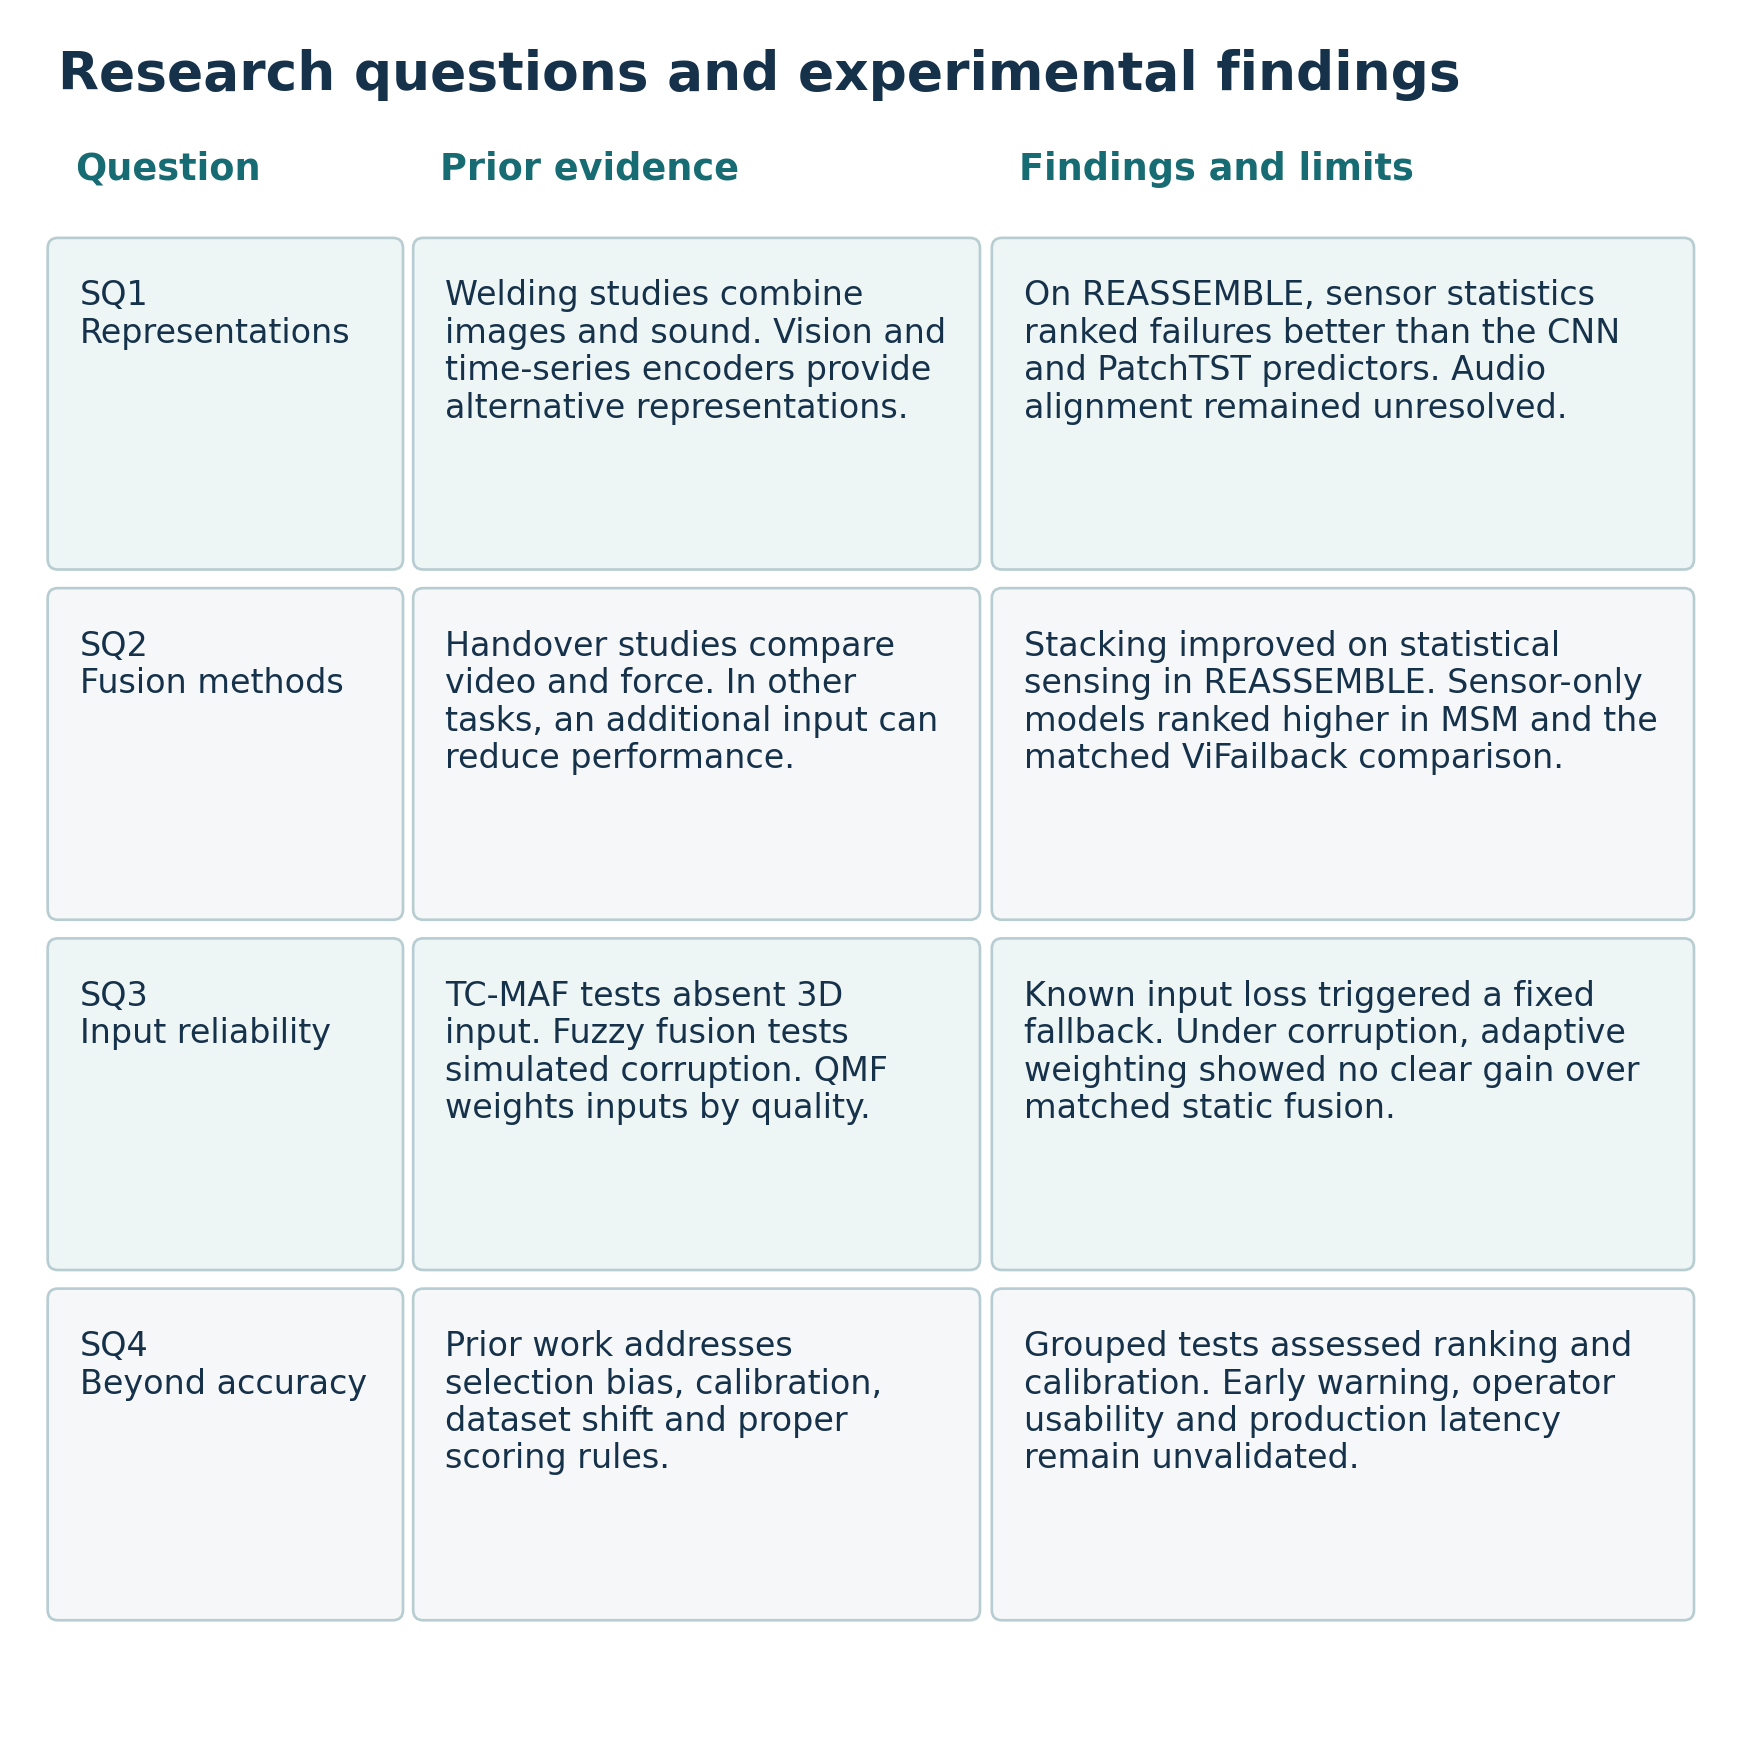
\includegraphics[width=\textwidth]{figures/gap_coverage.png}
\displaynote{The middle column summarises prior research. The right column gives the
corresponding experimental findings and limits.}
\end{figure}

\section{Threats to Validity and Unresolved Evidence}
Three features of the data limit a causal interpretation of architectural differences.
First, the target may only approximate the phenomenon of interest. PHM has no
independent quantitative tooth-damage reference, MSM's label mapping defines which
intervals count as abnormal, and some robotic outcomes remained ambiguous under visual
review. Second, the number of independently acquired units can be much smaller than the
number of predictions. Gear experiments, recording sessions, dates, tasks, and
participants capture different sources of dependence. Where identifiers were missing,
independence across those groups could not be verified. Third, several later analyses
revisited assessment populations examined during development. Intervals conditional on
fitted predictions and variation over a few seeds do not capture that selection history.

Preprocessing before the separate four-arm PHM loop limits attribution of its results to
architecture. In other experiments, differences in calibration, capacity, training
budget or corruption exposure accompanied architectural changes. Incomplete historical
PHM training-source lineage and unavailable ViFailback per-fit histories limit
independent reconstruction.\ev{Historical source and per-fit reconstruction limits}
{\EvidenceRef{E129}{}, \EvidenceRef{E130}{}, \EvidenceRef{E137}{}}
ViFailback's complete frozen/donor comparisons are supplemented by one-fold FULL20
evidence and separate hundred-epoch pilots; the adaptation contrasts remain
inconclusive. Whether the fine-tuning effect persists across the remaining task folds
and seeds is unknown, and corruption performance was unmeasured. The recorded forecast
was 43 additional GPU-days for the remaining FULL20 fits, with 47 days allowed including
variation and overhead. The central estimate scales the measured fitting rate by the
remaining split-specific workload. It is an estimated future runtime, not elapsed
GPU time or a confidence interval. This forecast covered
fine-tuning only (Section~\ref{sec:ch4-boundaries}).\ev{Completed adaptation scope and
recorded forecast}{\EvidenceRef{E113}{}, \EvidenceRef{E114}{}}
The literature synthesis covers the full texts available to a single reviewer.

Finally, the completed-window studies allowed the predictor to observe evidence near the
outcome. Synthetic blur, noise, or stream removal test specified interventions. They
give limited information about gradual calibration drift, unobserved timing faults, or
shifts to another physical machine. Transferring a predictor to an earlier decision time
or a different installation requires observations at that time and place.

\section{Implications for Multimodal System Design}
In a monitoring application, the intended decision determines what constitutes failure,
how it can be confirmed independently, and which observations arrive in time to be
useful. Evaluating each stream on the same held-out units establishes what it can
predict alone. Equal averaging and a fitted static combination then provide references
for testing whether context-dependent weights add value. When an instrument declares an
outage, the remaining predictor supplies a natural reference. When faulty values still
appear plausible, the relevant test is whether the gate recognises situations in which
trusting that stream would worsen the prediction.

A prospective return to welding could reserve whole welding sessions, collect an
independent weld-quality measure, and fix the prediction horizon before examining those
outcomes. On the same welds, exposure- and calibration-matched models could be assessed
for clean performance, known absence, degraded readings, timing error, and shifts
between operating conditions. Paired effects and a prespecified tolerance for
clean-performance loss would clarify the operational cost of any robustness gain. Such a
test would show whether the modest gain for completed assembly actions carries over to
weld-quality decisions.
